\documentclass[a4paper,10pt]{article}

% Hier die Nummer des Blatts und Autoren angeben.
\newcommand{\blatt}{11}
\newcommand{\autor}{Merlin Steuer, Till Schander, Lennart Bergmann}

\usepackage{hci}

\begin{document}
% Seitenkopf mit Informationen
\kopf
\renewcommand{\figurename}{Figure}

\aufgabe{16}

\subsection{Analyse}
blabla

\subsection{Design}
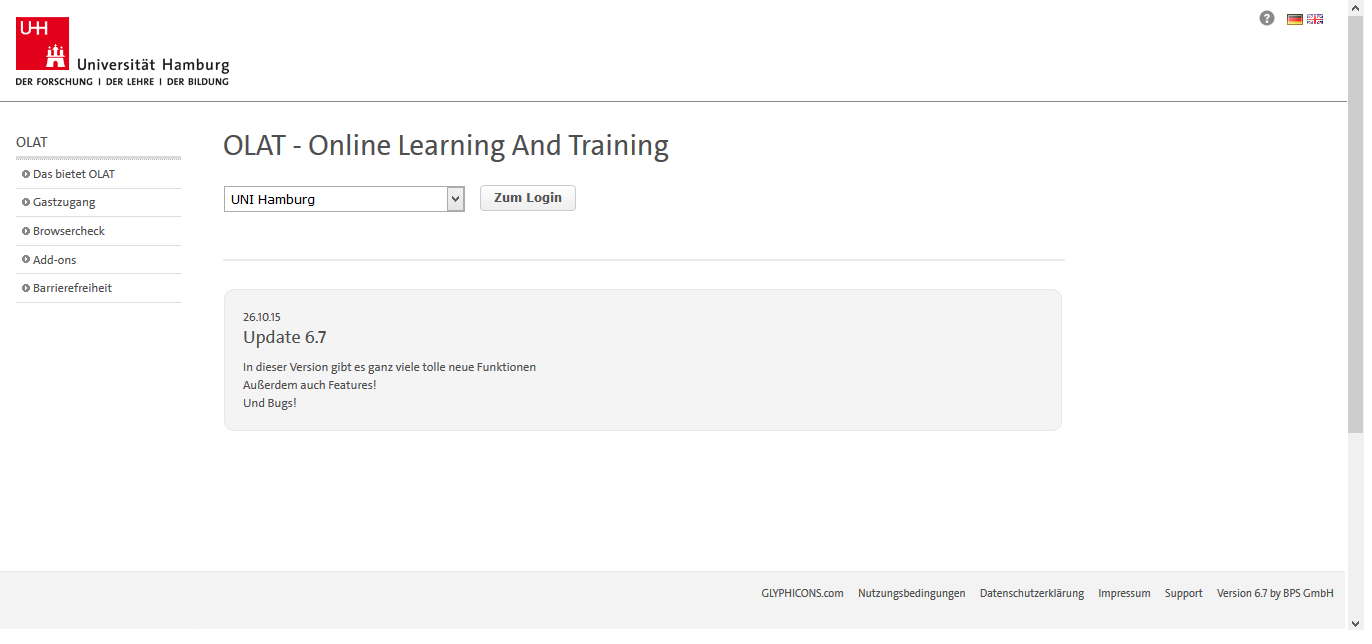
\includegraphics[scale=0.4]{images/login_seite.png}

Die Start-/Login-Seite wurde etwas entschlackt. Die Support-Emails kann man nun unter der Hilfe finden(Merging similiar options). Die Flaggen zur Sprachauswahl sind nun sofort beide sichtbar(exposing options), da ein Dropdown f�r zwei Optionen �berfl�ssig ist. Das Hauptaugenmerk liegt auf dem Login, da die meisten User daf�r die Seite besuchen.

Zudem haben wir uns entschieden den restlichen Platz f�r einen Newsstream zu nutzen, in dem wichtige Updates oder neue Features angek�ndigt werden k�nnen.


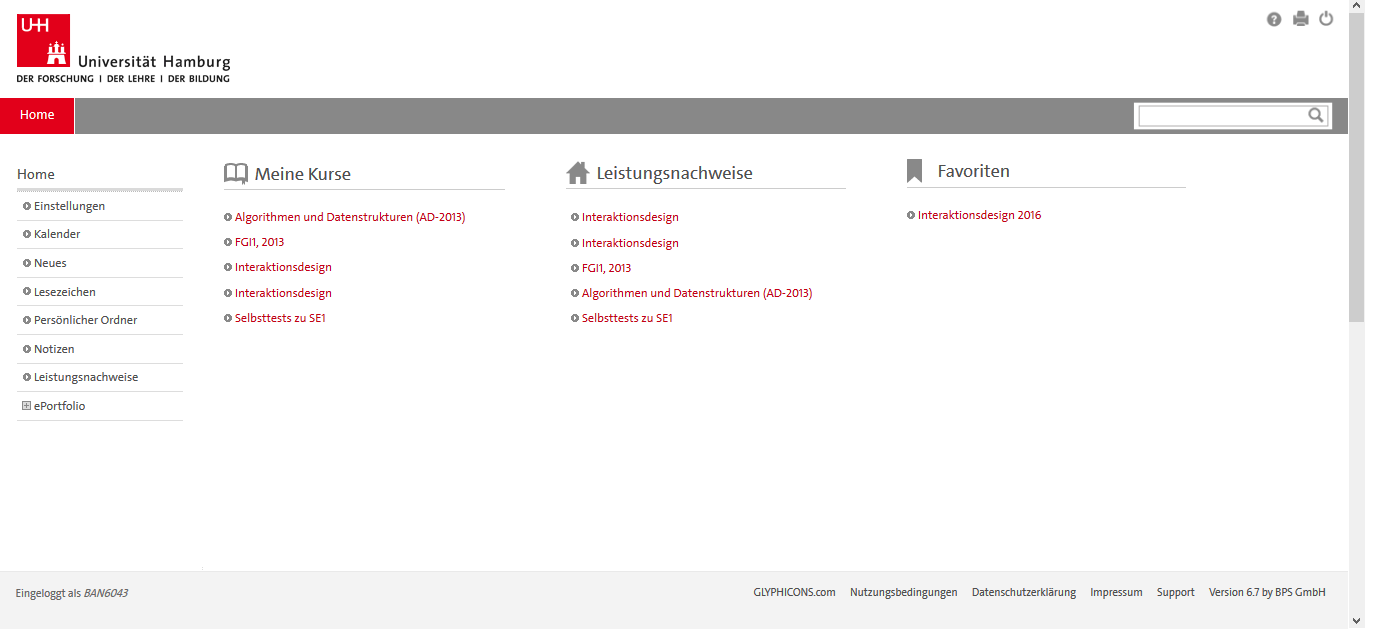
\includegraphics[scale=0.4]{images/wilkommen_seite.png}

Die Wilkommen-Seite wirkte sehr �berladen. Wir haben sie etwas aufger�umt und uns beim re-design auf die wichtigsten Aspekte beschr�nkt, auch wenn das Dashboard erhalten bleibt. Die meisten User werden OLAT aufrufen um in ihre Kurse zu gucken, oder ihre Bewertungen einzusehen, weshalb wir hierf�r einen "Clear Entry Point" geschaffen haben. Die Zeile f�r "Many Workspaces" bleibt nat�rlich erhalten, wird aber nur noch f�r ge�ffnete Kurse benutzt. Das Hauptaugenmerk liegt darauf, dem Nutzer einen simplere, eing�ngigere Oberfl�che zu pr�sentieren.

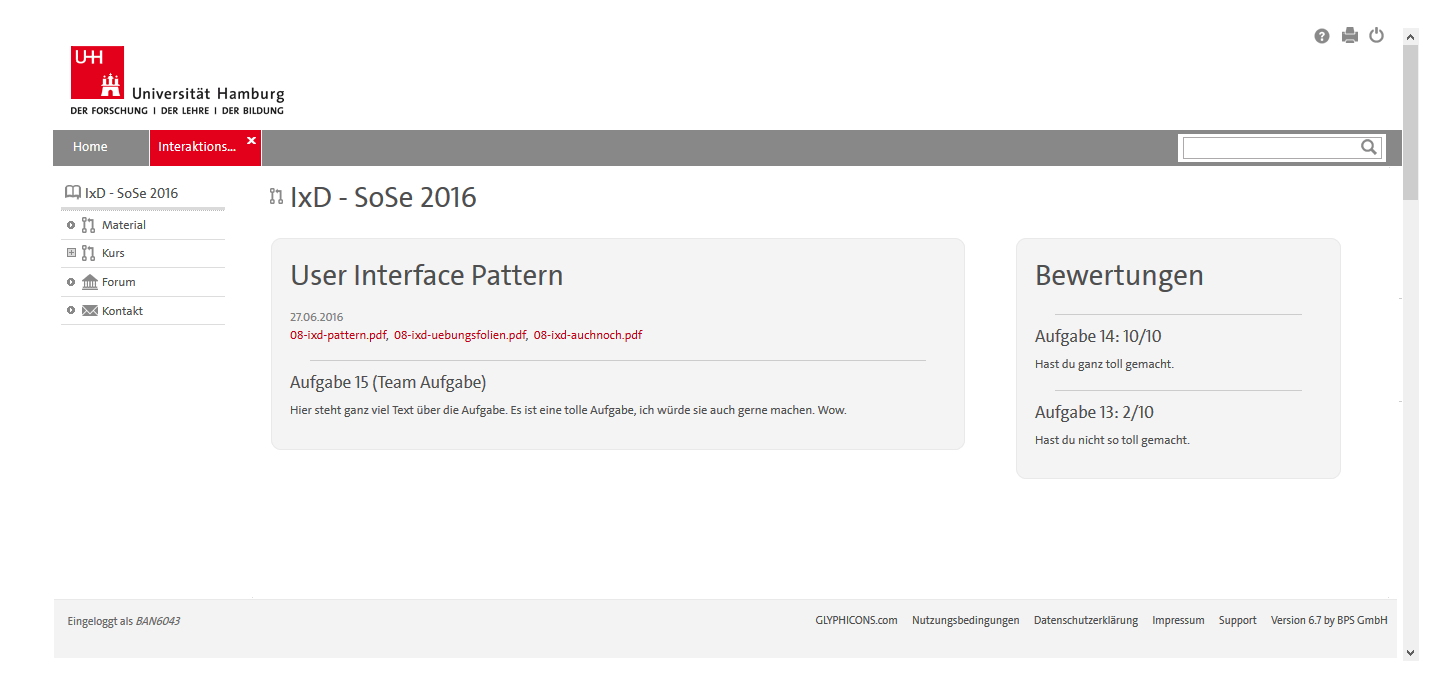
\includegraphics[scale=0.4]{images/ixd_seite.png}

Auch hier haben wir etwas aufger�umt. Es gibt nun schon auf der Startseite einen �berblick �ber die neusten Inhalte (Newsstream) sowie die letzten Bewertungen, da die meisten User diese Dinge am ehesten sehen wollen. Die bekannten Seiten bleiben nat�rlich erhalten(Alternative Views). Der "Ordner" hei�t jetzt "Material", damit der User wei�, was ihn hier erwartet. Auch wurden das Wiki, die Linkliste und das Literaturverzeichnis hierhin verschoben, um das Men� zu vereinfachen und zusammengeh�rige Optionen zu gruppieren. Zur besseren Verst�ndichkeit hei�t "Inhalt" jetzt "Kursinhalt" und "Email" wurde zu "Kontakt". Feature/Search/Browse.

Alle Bereiche haben oben links den Escape Hatch, und teilweise zus�tzlich noch den Home-Button. 

\subsection{Implementierung} 




\end{document}
